\documentclass{article}
    
\usepackage{Haust2017skil}

\title{Stærðfræðimynstur í tölvunarfræði \\ Skilaverkefni 4}
\author{}

\begin{document}
\maketitle

Skila skal þessu verkefni á vefnum \href{https://gradescope.com/courses/9487}{Gradescope}. Aðgangskóði fyrir námskeiðið er \textbf{9N834D}.

Gradescope tekur við .pdf skjölum. Frágangur á þeim skiptir máli. Þau skulu að vera hreinskrifuð í tölvu. Kerfi eins og \LaTeX, Google Docs og Microsoft Word geta búið til .pdf skjöl.

Samvinna á milli nemenda er eðlileg og æskileg. Hins vegar er afritun það aldrei. Miklu gagnlegra er að reyna við dæmin upp á eigin spýtur en að reyna að hala inn hærri einkunn með því að skila inn lausnum annarra.

Telji nemandi að mistök hafi verið gerð við yfirferð skal tilkynna slíkt á Gradescope.

\section{Kafli 3.2}

\question

Sýnið að $\frac{x^3+2x}{2x+1}$ sé $O(x^2)$.

\paragraph{Í bók:} 3.2.6 í báðum útgáfum

\question

Látum $k$ vera jákvæða heiltölu. Sýnið að $1^k + 2^k + \ldots + n^k$ sé $O(n^{k+1})$.

\paragraph{Í bók:} 3.2.18 í Icelandic/International, 3.2.14 í Global

\question

Byggt á spurningu á lokaprófi 2016.

\textbf{(Ísl)} Raðið föllunum 
\[
    \sqrt{n}, 9^{999} n, 2^n, 10\log n, n!, 1000 n^2, 2 n^{1000}, n \log n
\]
í runu svo að hvert fall sé í stóra-O af þeim sem á eftir koma.

\textbf{(En)} Write the functions above in a sequence so that each function is big-$O$ of the later functions in the sequence.

\section{Kafli 3.3}

\question

Regla Horners er skilvirk leið til að reikna gildi margliðu. Eftirfarandi sauðakóði reiknar gildi margliðunnar $a_nx^n + a_{n-1}x^{n-1}+\ldots+a_1x+a_0$ í $x = c$:

\begin{center}
    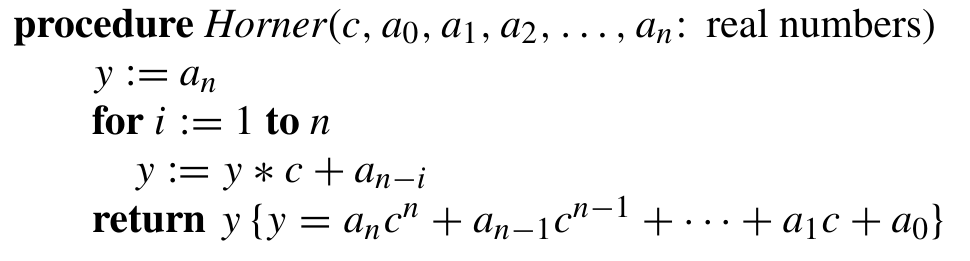
\includegraphics[width=0.6\textwidth]{horner}
\end{center}

\begin{itemize}
    \item[a)] Notið reglu Horners til að reikna gildi $3x^2+x+1$ í $x=3$
    \item[b)] Hversu margar margfaldanir og hversu margar samlagningar þarf regla Horners til að reikna gildi $n$-ta stigs margliðu í ákveðnum punkti? (Ekki telja þær aðgerðir sem gæti þurft til að uppfæra gildið $i$.)
\end{itemize}

\paragraph{Í bók:} 3.3.14 í Icelandic/International, 3.3.10 í Global

\question

Þurfi reiknirit sem leysir ákveðið vandamál $f(n)$ aðgerðir, hversu stórt vandamál væri hægt að leysa á einum degi á tölvu sem framkvæmir eina aðgerð á $10^{-11}$ sekúndum, fyrir eftirfarandi $f(n)$?

\begin{itemize}
    \item[a)] $\log_2 n$
    \item[b)] $1000n$
    \item[c)] $n^2$
    \item[f)] $2^n$
\end{itemize}

\paragraph{Í bók:} 3.3.16 í Icelandic/International. Ekki til staðar í Global edition, svipar til 3.3.11

\question

Hversu langan tíma þarf reiknirit til að leysa vandamál ef það þarf $2n^2+2^n$ aðgerðir til að leysa vandamál af stærð $n$, sé reikniritið keyrt á tölvu sem framkvæmir eina aðgerð á $10^{-9}$ sekúndum? Svarið fyrir eftirfarandi gildi á $n$:

\begin{itemize}
    \item[a)] 10
    \item[d)] 100
\end{itemize}

\paragraph{Í bók:} Dæmi 3.3.18 í Icelandic/International, 3.3.12 í Global



\end{document}
